\documentclass[11pt]{article}

\usepackage{graphicx}
\usepackage{multirow}
\usepackage{amssymb}
\usepackage{amsmath}
\usepackage[left = 2cm, right = 2cm, top = 2cm, bottom = 2cm]{geometry}
\usepackage{hyperref}
\usepackage{xcolor}
\usepackage{physics}
\usepackage{soul}
\usepackage{subcaption}
\usepackage{verbatim}
\usepackage{listings}

\lstset{basicstyle=\ttfamily,
columns=fullflexible,
frame=single,
breaklines=true,
postbreak=\mbox{\textcolor{red}{$\hookrightarrow$}\space},
language=C++}

\definecolor{red2}{RGB}{255, 49, 49}
\definecolor{green2}{RGB}{144, 238, 144}
\definecolor{purple2}{RGB}{150, 111, 214}
\newcommand{\hlyellow}[1]{{\sethlcolor{yellow}\hl{#1}}}
\newcommand{\hlgreen}[1]{{\sethlcolor{green2}\hl{#1}}}
\newcommand{\hlred}[1]{{\sethlcolor{red2}\hl{#1}}}
\newcommand{\hlpurple}[1]{{\sethlcolor{purple2}\hl{#1}}}

\bibliographystyle{unsrt}%abbrv} % We choose the "plain" reference style

\title{Notes on Weightfield2 - Resistive Silicon Detectors}
\author{Danush Shekar\\ Supervised by Dr. Zhenyu Ye}
\date{\today}

\begin{document}

\maketitle
\tableofcontents

\newpage

%\abstract{}%This is my attempt in saving an account of all tips/tricks, notes, and discussions of the simulation tools I have used (mostly related to HEP simulations). In theory, this is also a note to questions and answers I encountered while I studied the subject, and that this notebook should serve as a reference for the doubts my mind stumbles upon in the future.}

\subsection*{Colour legend}
This document will follow a highlighting scheme where text highlighted in different colors mean the following:
\newline
\hlyellow{Yellow coloured text} - Doubts, or sentences that are to be clarified/understood later.\newline
\hlgreen{Green coloured text} - Some takeaways.\newline
%\hlred{Red coloured text} - Mistakes/typos.\newline
\hlpurple{Purple coloured text} - Interesting and unique points, that often are not mentioned explicitly in textbooks/literature.

\section{About}
The WeightField\footnote{The manual for this (first) version can be found at \href{http://personalpages.to.infn.it/~cartigli/Weightfield2/Manual_files/Manual_Weightfield.pdf}{here}} (WF) software is a tool used to simulate a variety of silicon detectors: different versions have been updated over time to study a variety of silicon sensors. As the name suggests, the WeightField2\footnote{Main link to manuals/guides - \href{http://personalpages.to.infn.it/~cartigli/Weightfield2/Manual.html}{http://personalpages.to.infn.it/~cartigli/Weightfield2/Manual.html}.} (WF2) software is the second iteration of WF. An important step in detector simulations is the calculation of the electric and weighting fields, and only then the induced current calculations follow. For WF and WF2, the weighting potential is calculated by solving for the Laplace equation using numerical methods (which also involves interpolation), and the induced current is calculated using the Shockley-Ramo theorem. %An important piece of information that one should keep at the back of your head while using this software is that ``the backplane is at the bottom and the strips on the top edge with the readout strip being always centered".

WF2-RSD (WF2 - Resistive Silicon Detectors) is a version of software that rolled-out after WF2. The primary objective of this tool is to simulate RSDs (or also known as AC-LGADs). In some parts of the code, I believe (and this is a personal opinion) that quantities being calculated are mimicking the experimental results and not truly simulating the physics behind such processes. This might also partly be because we still don't know what is happening in AC-LGADs, for example, the signal induction to the AC pads.
\newline
Two references that explain some working principles of WF2-RSD are \cite{wf2-rsd-working-principles} and \cite{Tornago2021}. The former discusses the models used to calculate the charge sharing (among different pads) and signal delay and the later is a more detailed article on the same.
\newline
WF2-RSD differs from WF2 in the following aspects:
\begin{enumerate}
    \item Resistive layer - capability to simulate a resistive layer with a user-defined resistivity.
    \item Addition of circular pads (instead of strips) by default - User can change number of pads, and packing (square and hexagonal packing of the pads).
    \item Naturally, the signal induction calculation has been updated, and the signal sharing model (Logarithmic attenuation model \cite{Tornago2021}) has also been included.
\end{enumerate}

\section{Input Panel Variables/Quantities}
The WF2-RSD front-end has many parameters and sections for plots and an example of the same can be seen in Figure \ref{fig:3x3_pad_field}. This section walks the reader through what each section is for, along with a brief description of the quantities/results involved.
\subsection{Panel: Detector properties}
There are 3 detector types under the ``\textbf{Type}'' section (namely Silicon, diamond, and SiC). This refers to the type of material the detector is made of. Each option would involve different values for quanitities like dielectric constant, (e/h) mobilities, etc.
\newline
Since we are dealing with AC-LGADs, in the next section ``\textbf{Doping Type}'' would only involve choosing n-type strips (referring to the n+ layer) and p-type bulk.
\newline
The options involved with the ``\textbf{Dimensions}" section and their description are as follows:
\begin{enumerate}
    \item Stacked - Switching-on this option will go from rectangularly packed pads (default) to hexagonal packing of the pads.
    \item Number of pads - The number of pads that will be present in the sensor geometry. A screenshot of the simulation window/screen for 2 different pad numbers are shown in Figure \ref{fig:ss_number_of_pads}.
    \begin{figure*}[h!]
        \centering
        \begin{subfigure}[t]{0.99\textwidth}
            \centering
            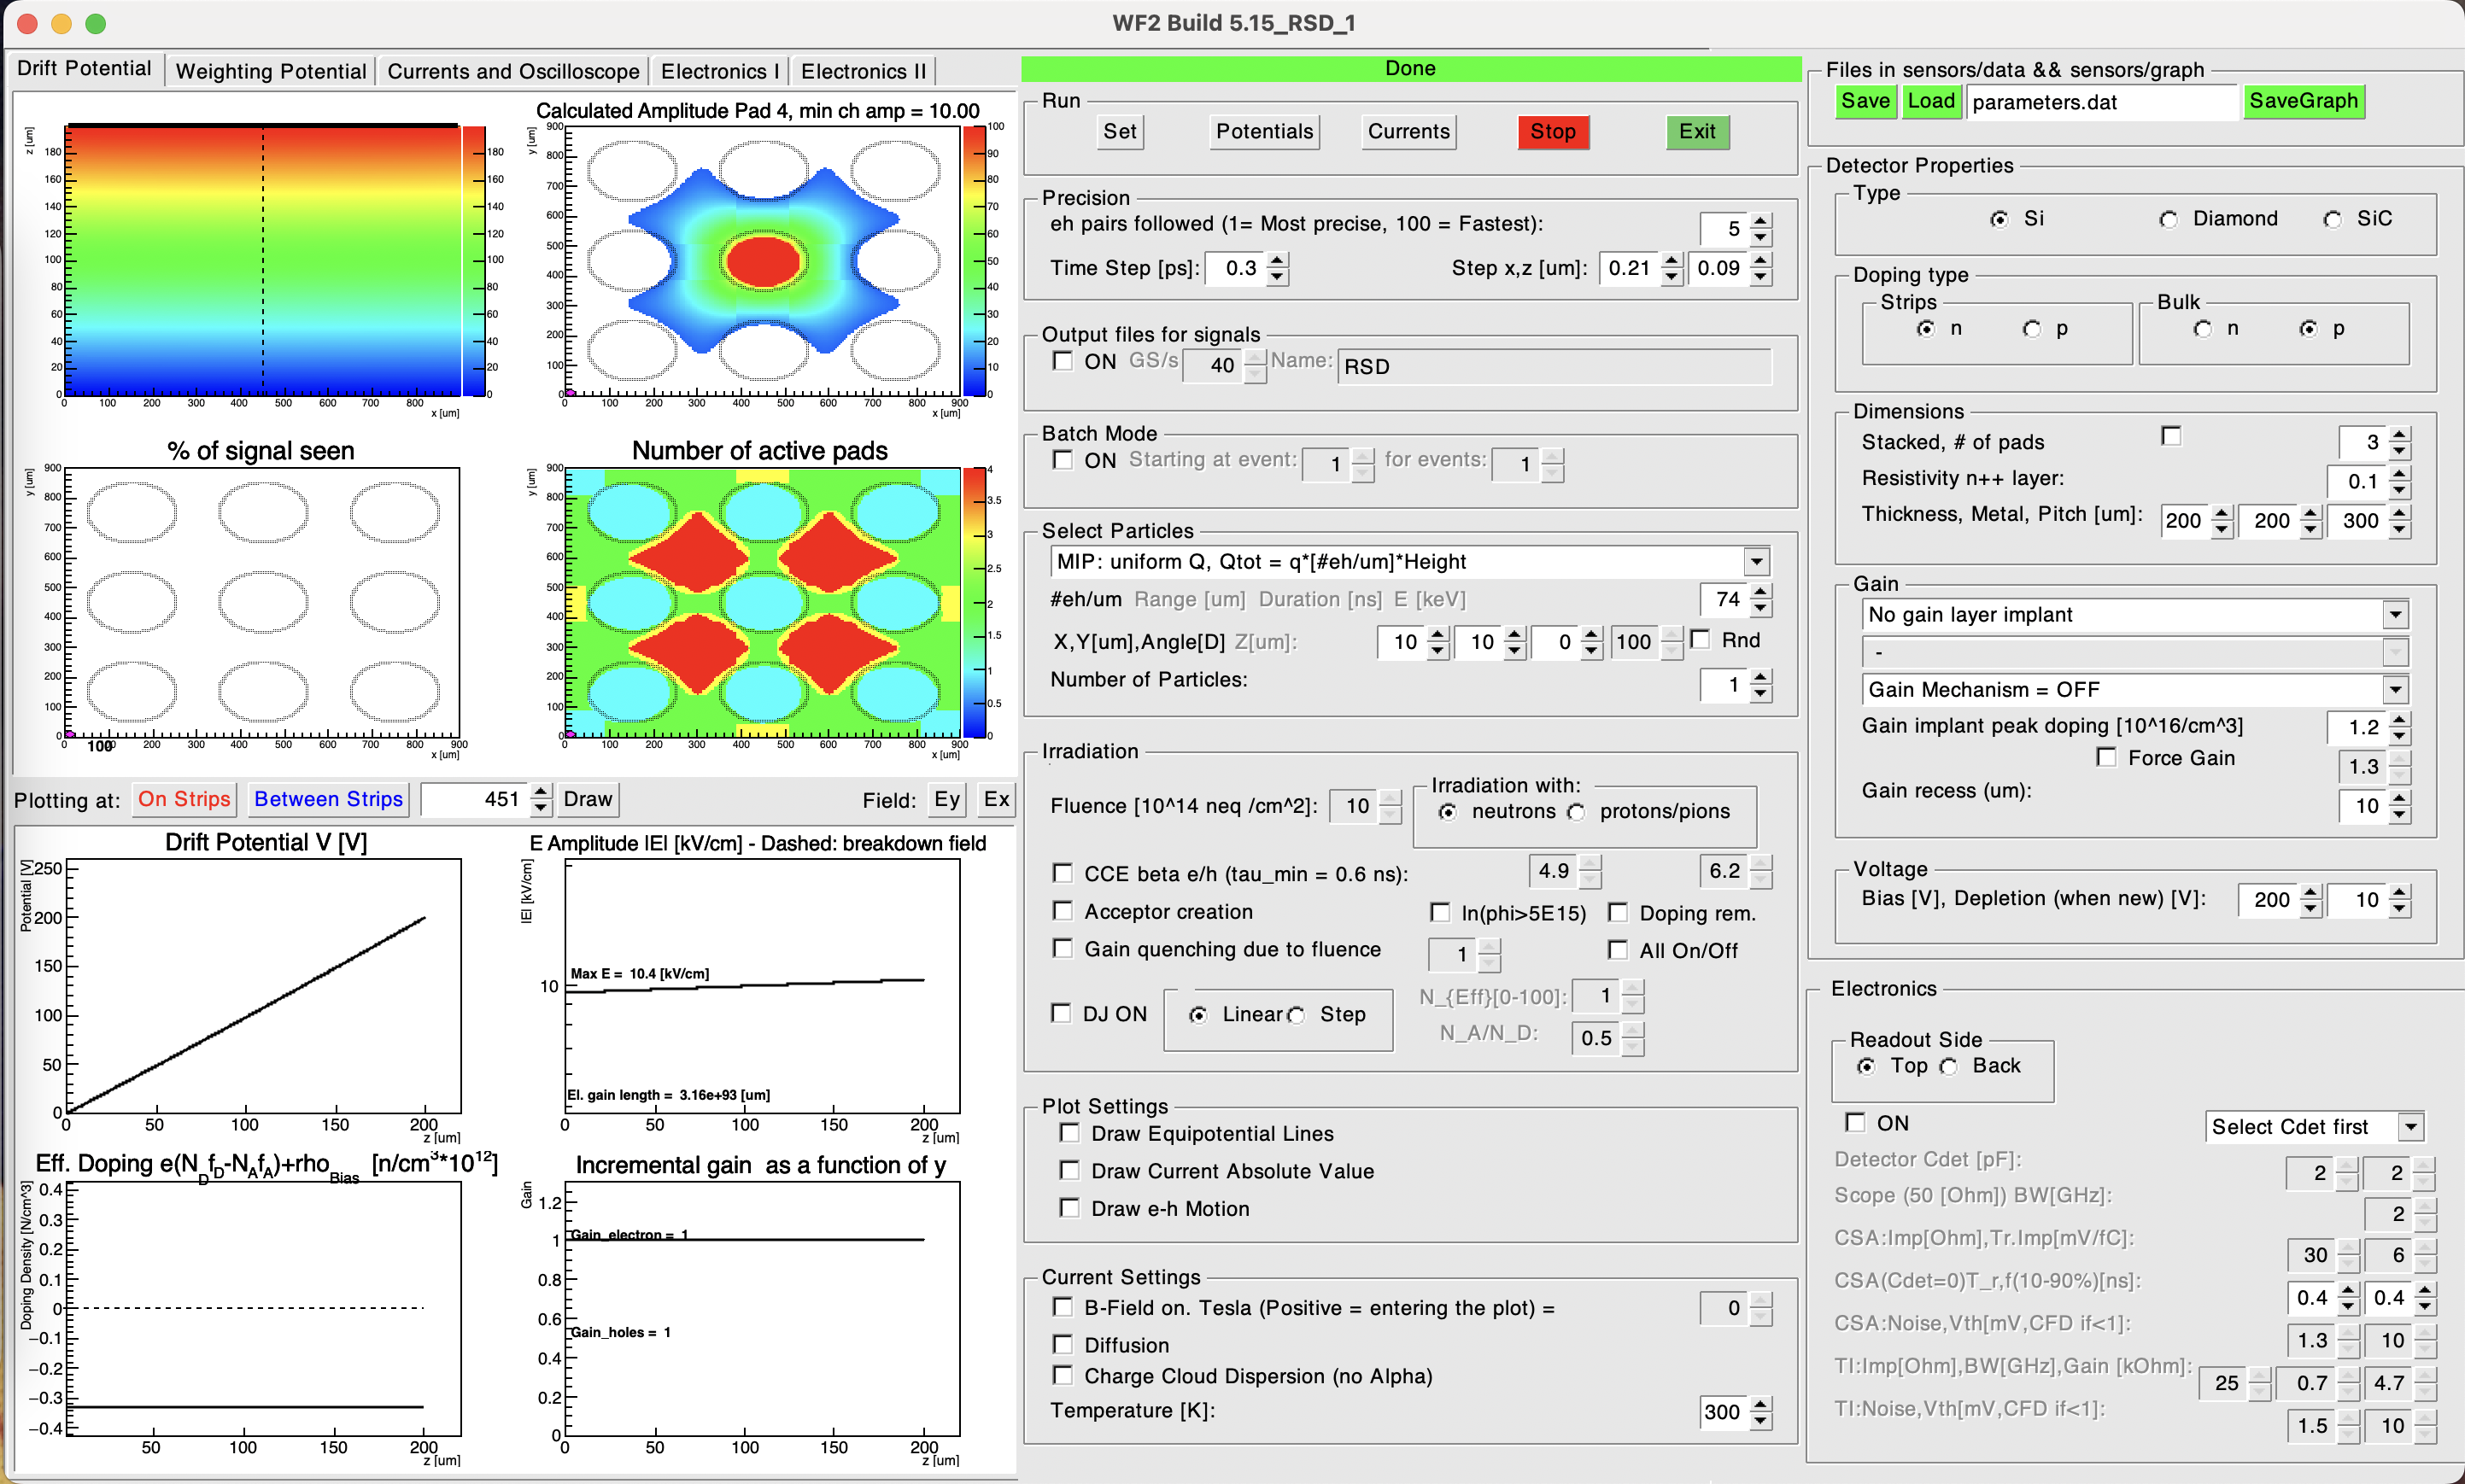
\includegraphics[width=5in]{Images/3x3_pad_structure.png}
            \caption{}
            \label{fig:3x3_pad_field}
        \end{subfigure}%

        \begin{subfigure}[t]{0.99\textwidth}
            \centering
            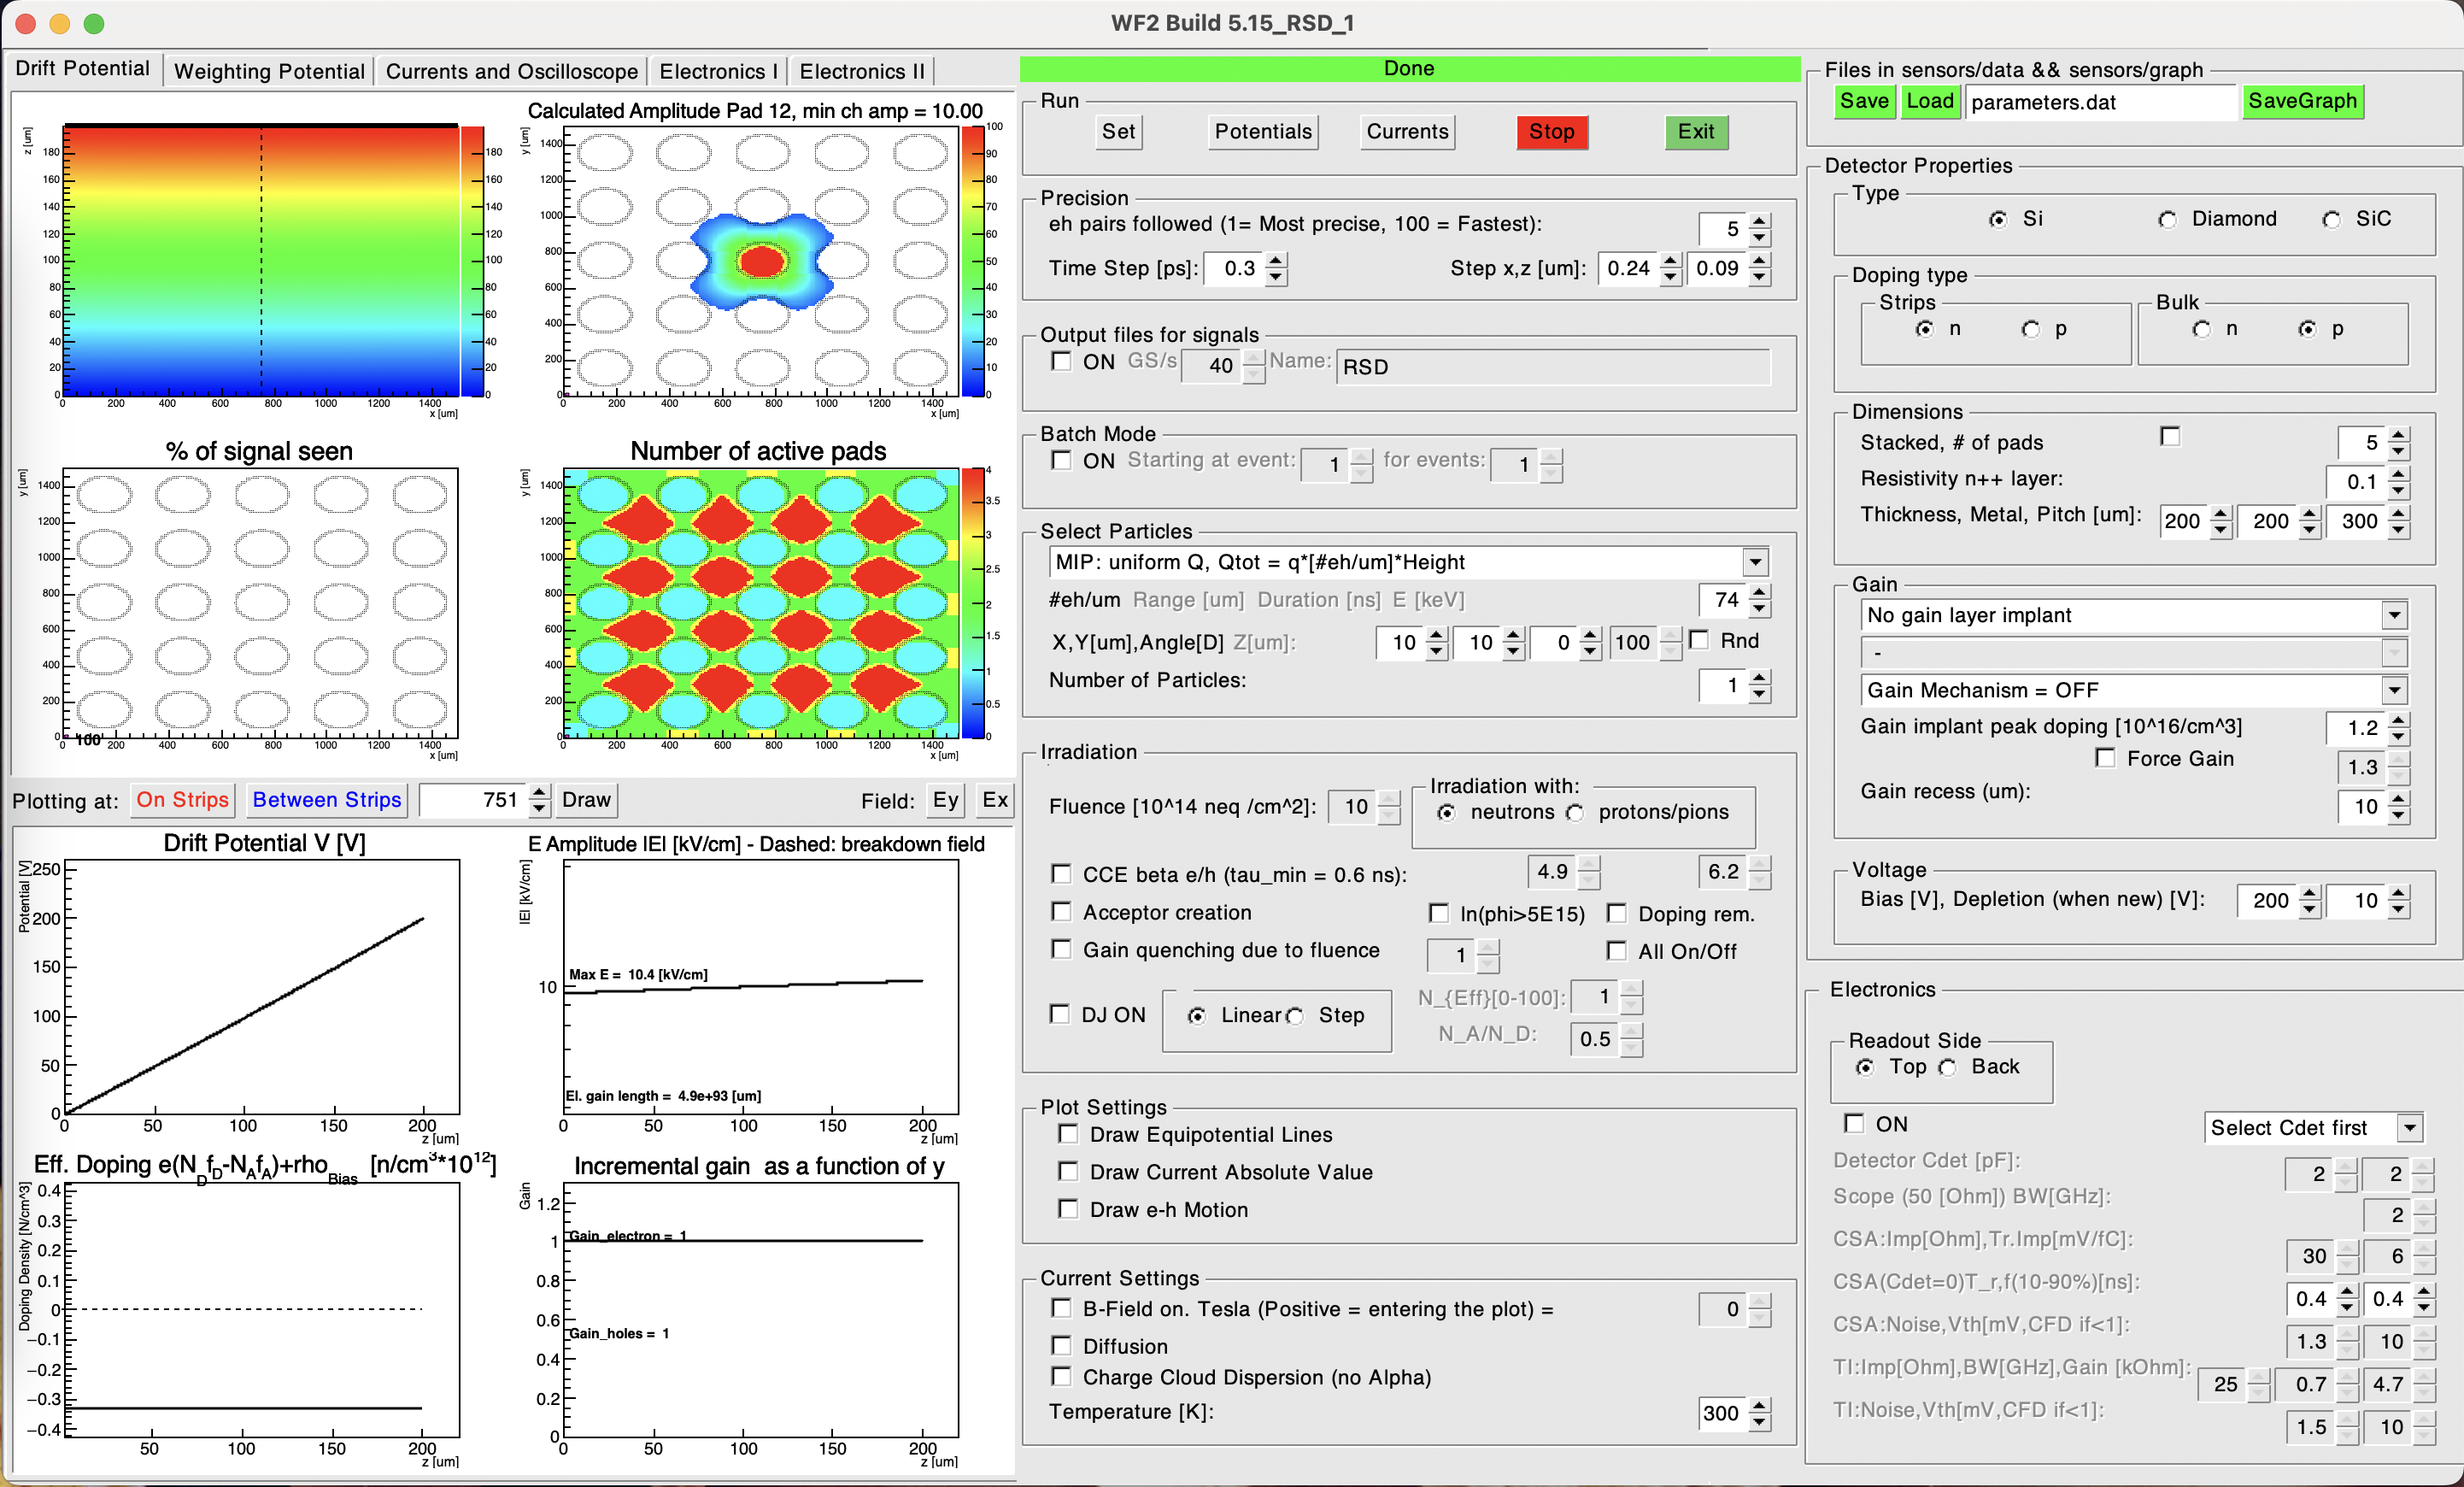
\includegraphics[width=5in]{Images/5x5_pad_structure.png}
            \caption{}
            \label{fig:5x5_pad_field}
        \end{subfigure}
        \caption{Software settings and results for (a) 3 $\times$ 3 and (b) 5 $\times$ 5 pad structures.}
        \label{fig:ss_number_of_pads}
    \end{figure*}
    \item Resistivity n+ layer - Refers to the resistivity of the n+ layer. The sheet resistance is set to 1k$\Omega$/$\square$.\hlyellow{Check for changes in current for different resistivity values}.
    \item Thickness - The thickness of the detector (if one observes carefully, there is no consideration of pad thickness - which does not affect the potential values under the pads, i.e. in the detector volume). The value that is assigned to this quantity is the thickness of the bulk substrate (active volume - where the primary charges are created by an incident radiation). The top left plot under drift-potential plots is the cross-sectional plot of the electric potential across the detector.
    \item Metal - The diameter of the circular pads (\href{http://personalpages.to.infn.it/~cartigli/Weightfield2/WF2_RSD_files/CERN_Cartiglia_modified.pdf}{Reference} - slide 16).
    \item Pitch - The distance between 2 adjacent pads. Should be greater than the metal diameter ofcourse.
\end{enumerate}
The options' description for the ``\textbf{Gain}" section:
\begin{enumerate}
    \item Dopant material - Options include Boron, Boron+Carbon, Gallium, and Gallium+Carbon. The addition of Carbon is known to improve radiation hardness \cite{ferrero-radiation-hardness}.
    \item Gain layer uniformity+position: 
        \begin{itemize}
            \item Uniform corresponds to a uniform doping concentration. 
            \item The numbers that follow after the setting/configuration is the position of the electrode from which the gain layer will be implanted. 
            \item LD corresponds to Low-Diffusion [sensors with, say a Boron gain layer that were exposed to a reduced thermal load during production to minimize the diffusion of Boron (Boron low-diffusion)] \cite{ferrero-radiation-hardness}. See \href{https://indico.cern.ch/event/806731/contributions/3516709/attachments/1926118/3188326/191013-VERTEX-RD50-mmoll-acceptor-removal.pdf}{this} link for a better picture.
            \item The number that precedes the configuration refers to the identification tag/name given to the sensor version (Eg - 3.1 refers to the HPK-3.1 sensors made by HPK) \cite{jadhav-sensor-variation, jin-sensor-variation}.
            \item There is one option with the word `Epi': it refers to an Epitaxial substrate. \hlyellow{Although as the setting suggests that the depth of the layer is 3 $\mu$m, but the effective doping plot shows that the layer begins somewhere between 199 $\mu$m and 200 $\mu$m (a small offset is also present for other implant settings).}
        \end{itemize}
    \item Forced gain value - According to Cartiglia's website manual, one can forcefully set a gain value, which in-turn removes the dependance from the bias voltage. A hint along the same direction to what is happening with this step can be understood from Figure 10 in\cite{ferrero-radiation-hardness}.
    \item Impact-ionization models - Simulation of the gain mechanism through various models. The user has a choice between 4 models, namely, Van Overstraeten model, Okuto-Crowell model, Bologna model, and Massey-LGAD model. Table \ref{tab:impact-ionization-models} summarises some differences between these 4 models.
\end{enumerate}
\begin{table}[!h]
    \centering
    \begin{tabular}{|c|c|c|}
        \hline
        Sensor Version/Name & Thickness & Implant level        \\ \hline
        HPK-1.2             & 35$\mu$m & Shallow (1.1-1.5$\mu$m) \\ \hline
        HPK-3.1             & 50$\mu$m & Deep (1.3-1.9$\mu$m)    \\ \hline
        HPK-3.2             & 50$\mu$m & Deeper (1.9-2.3$\mu$m)    \\ \hline
    \end{tabular}
    \caption{Comparison of some parameters of 3 types of sensors used in WF2-RSD simulations. The numbers in paranthesis in the Implant level column are ones used in WF2-RSD.}
    \label{tab:hpk-sensor-parameters}
\end{table}
\begin{table}[h]
    \centering
    \resizebox{5in}{!}{%
    \begin{tabular}{|c|c|cc|}
    \hline
    \multirow{2}{*}{Model} & \multirow{2}{*}{Year Introduced} & \multicolumn{2}{c|}{Valid over:}                                                 \\ \cline{3-4} 
                           &                                  & \multicolumn{1}{c|}{Electric field (x10$^5$   Vcm$^{-1}$)} & Temperature (K) \\ \hline
    Van Overstraeten & 1970 & \multicolumn{1}{c|}{1.75 - 6.4} & NIL        \\ \hline
    Okuto-Crowell    & 1975 & \multicolumn{1}{c|}{1.0 - 10.0} & Around 300 \\ \hline
    Massey           & 2006 & \multicolumn{1}{c|}{2.0 - 8.0}  & 14 - 420   \\ \hline
    Bologna          & 1999 & \multicolumn{1}{c|}{0.5 - 6.0}  & 300 - 700  \\ \hline
    \end{tabular}%
    }
    \caption{Some differences between the impact-ionization models that can be used in WF2-RSD.}
    \label{tab:impact-ionization-models}
\end{table}
\cite{arcidiacono-irradiation} found that the gain layer produced in Low Diffusion (LD-narrower layer profile) is more radiation resistant than the High Diffusion (HD) type; (ii) the co-implantation of carbon in the gain layer volume improves by a factor of $\approx$2 the radiation resistance. \cite{ferrero-radiation-hardness} additionally found that Gallium doping is less radiation resistant than Boron doping, and that narrower gain layer implants are more radiation resistant than wider implants.

\subsection{Panel: Electronics}
\begin{enumerate}
    \item Detector capacitance
    \item Oscilloscope bandwidth
    \item Charge Sensitive Amplifier:
    \begin{itemize}
        \item Input resistance
        \item Rise time/ fall time
        \item Trans-impedance
        \item Noise and threshold voltage
    \end{itemize}
    \item Broad-Band Amplifier (renamed as TI in WF2-RSD):
    \begin{itemize}
        \item Bandwidth and gain
        \item Noise and threshold voltage
    \end{itemize}
\end{enumerate}
Changing parameters of the Charge Sensitive Amplifier (CSA), changes the (Broad-Band) BB amplifier output. This probably suggests that we are looking at a readout `chain' (sensor $\rightarrow$ CSA $\rightarrow$ TI) and not two independent amplifier outputs. \hlyellow{Although this is not evident when looking at the code for how these two quantities are calculated.}
\newline
First, some CAS and TI amplifier parameters were investigated: the noise and threshold voltages (of both CSA and TI) were varied to study what changes they introduce in the final output. A noise voltage of 0.001, 0.1, 1.5, 10, and 50 mV (while other parameters were kept constant) did not show any visible changes in the outputs. The same was done for threshold voltage for 0.001, 0.1, 1, 10, and 50 mV (while other parameters were kept constant) and no visible changes were seen in the output. \hlyellow{Understanding how noises are calculated and inculcated into the final output is yet to be done.}

For the entirety of this report, unless mentioned otherwise, the legend for the plots from the ``Currents and Oscilloscope" tab (which includes and is not limited to the signal from the AC-pads and the oscilloscope) is shown in Figure \ref{fig:wf2-legend}. If there are other colored lines in the plots than what is seen in the figure, that represents the signal seen by the remaining AC-pads as only colors for two AC-pads are shown in the legend.

\begin{figure}[h]
    \centering
    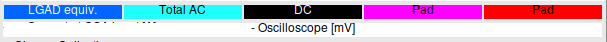
\includegraphics[width=4in]{Images/Legend.png}
    \caption{The legend for the plots containing the response of the AC-pads, DC contact, and the oscilloscope (thin-grey line).}
    \label{fig:wf2-legend}
\end{figure}

\subsection{Panel: Select Particles}\label{sec:select-particles}
This subsection has been organised according to the particle type, as each particle type have a different set of options that can be configured. The user has an option to choose from Minimum Ionizing Particles (MIPs), X-Rays, Lasers, and a current pulse.
\begin{enumerate}
    \item MIPs - User can define the incident position of the MIPs and the number of MIPs. The user can select the type of energy deposition:
    \begin{itemize}
        \item Uniform/Non-uniform energy deposition - fixes the number of electron-hole pairs deposited per $\mu$m.
        \item Landau - An energy deposition that follows a Landau distribution. One can also have a MIP passing through the detector from left to right (Edge MIP Landau), instead the default top to bottom.
    \end{itemize}
    \item Laser - Options can let the user decide if the laser has to enter the detector from top-down, or down-top, or left-right (Edge)
\end{enumerate}
More details on the same can be found in \cite{WF2-incident-particles-cenna}.
\newline
Edge-TCT measurements (shooting laser beams left-right) are used to measure the depletion depth for a certain voltage bias \cite{moll-acceptor-removal}.

\subsection{Panel: Batch mode and output files}
Running the simulation on a batch mode essentially repeats one run of the simulation many times. One aspect of the results that is different is the plot from the electronics: a single run will show the waveforms of the CSA and the TI, whereas a batch mode run will produce histograms on resolutions that is yet to be understood.
\newline
WF2-RSD provides an option to save the output files, the contents of which were not fully sufficient to produce the figures in Section \ref{sec:full_analysis}. Thus, the source code was modified to store/save the results in a relevant format.

\subsection{Panel: Plots}
A brief outline of the plots made in the ``\textbf{Drift Potential}" section is as follows:
\begin{enumerate}
    \item XZ potential contour (top left) - Contour plot of electric potential across the XZ plane for a Y-plane. Apparently, since we have uniform doping and a uniform active region, this plot should be similar for all Y-values.
    \item Calculated amplitude plot (top right) for say, pad `A' and minimum charge amplitude = say `B' - Plot across the XY plane that signifies when a particle/radiation passes through a point in that XY-plane, how much of the amplitude reached pad `A'. Signal amplitude below `B' is not considered.
    \item \% of signal seen (bottom left) - For the incident particle(s)/radiation incident at the given position (marked with a purple dot in plot), the percentage amount of the signal reaching nearby pads is represented in this plot. Do \textbf{note} that the percentage value is shown below the pad, and not above it. Sometimes two numbers are displayed outside the plot-area, just poor formatting.
    \item Number of active pads (bottom right) - A plot on the XY-play, such that, for incoming particle(s)/radiation on a certain point in the plot, how many pads will pick up the signal (this number is given by the z-colour-axis).
\end{enumerate}

\section{Brief review of the source code}

A few sections of code that are important to know were understood and the same have been described in the following sub-sections. These sub-sections will be updated as more sections of the source code is decoded/interpreted.

\subsection{Charge and current generation}
Every electron/hole generated, an C++ object (from class \texttt{Carriers})is created that contains information like charge, position, velocity, etc. Most of the charge-generation and current-calculations are done in the file Carriers.cxx. As mentioned in Section \ref{sec:select-particles}, depending on the charge deposition mechanism the user chooses, an array called \texttt{NPairsPer5Micron} is updated with the number of primary charges per 5 $\mu$m in the sensor active volume, and objects of the \texttt{Carriers} class are created with position and charge information. There is a limit on the number of charges WF2 can track because there is a (large) fixed number of objects defined. 
\newline Mobilities are defined and at each time-step, for each particle, the velocities and positions are updated (using the electric field and mobility values). The positions involve both updated from a diffusion and drift component. Then a temporary induced current value is updated based off of this movement for each charge that is calculated using Ramo's theorem. If the charge(s) is in the gain layer region, the user-defined gain model is used and new objects are added to the \texttt{Carriers} accordingly. One of the snippets that shows the calculation of the temporary current using Ramo's theorem from electrons (\texttt{ie[]}) and holes (\texttt{ih[]}) is shown below:
\begin{lstlisting}
    if (carriers[j].GetCharge()==-1)
        ie[i]+=(-1)*(-1)*chargescale*ECHARGE*(wfield[PosBiny][PosBinx].GetFieldx()*carriers[j].GetVx() + wfield[PosBiny][PosBinx].GetFieldy()*carriers[j].GetVy());   
	else
		ih[i]+=(-1)*chargescale*ECHARGE*(wfield[PosBiny][PosBinx].GetFieldx()*carriers[j].GetVx()+ wfield[PosBiny][PosBinx].GetFieldy()*carriers[j].GetVy());
\end{lstlisting}
After this, the final current is calculated through a convolution of the (temporary) induced current and an exponential function (kernel). The snippet of code that does the same is as shown below:
\begin{lstlisting}
    for (int i=0;i<IMax-1;i++) //AC discharge
	{
	    for (int ll = 0; ll<IMaxSh-i;ll++)  // valid only up to IMaxSh 
	    {
		    CurrentStep =  itot[i]*TIMEUNIT/(tau_RSD)*TMath::Exp(-ll*TIMEUNIT/(tau_RSD));
		    itotQ[i+ll] += -CurrentStep; //final current from the AC pads
		    iDC[i+ll] += CurrentStep; // The current for DC contact
	    }
	}
\end{lstlisting}
The variable \texttt{tau\_RSD} involves the resistance and capcitance of the n+ layer and the oxide layer respectively.
\newline
The output of the oscilloscope, trans-impedance(/broad-band) amplifier, and the charge-sensitive amplifier (/shaper) can be summarised by the following snippet:
\begin{lstlisting}
    for (int ll = 0; ll<IMaxSh-i;ll+=Step)  // valid only up to IMaxSh 
    {
        Iout_C50[i+ll]   += (Qdif_Shaper)/tau_scope*TMath::Exp(-ll*TIMEUNIT/tau_scope); //Qdif_shaper is essentially the charge from the total induced current
        Iout_BB_RC[i+ll] += (Qdif_Shaper)/tau_BBA*TMath::Exp(-ll*TIMEUNIT/tau_BBA); //Input current to the BBA, convolution with BW

        Vout_scope[i+ll] = 50*Iout_C50[i+ll]; // Output Voltage Scope
        BBGraph[i+ll] = 1e+3*BBGain*Iout_BB_RC[i+ll]; // Output Voltage BBA

        // saturation of pre-amp output
        if ( fabs(BBGraph[i+ll])>800)  BBGraph[i+ll] = 800*BBGraph[i+ll]/fabs(BBGraph[i+ll]);
        //
        if (! gui->GetNA62On())		    
            {
            ShaperOut_Q[i+ll] += TauFall/(TauFall+TauRise_CSA)*Qdif_Shaper*(TMath::Exp(-ll*TIMEUNIT/TauFall)-TMath::Exp(-ll*TIMEUNIT/TauRise_CSA)); // [Q] HS eq 4.3 This is the shaper
            }
        }
\end{lstlisting}
Ofcourse, there are some further improvisations that we will not get into, for examples, a finite linear interpolation that is done to the voltage outputs of the oscilloscope and amplifiers, there are further plots produced from these quantities, etc.

\subsection{Signal sharing model(s)}
Signal-sharing is a unique feature that AC-LGADs display and WF2-RSD simulates this effect by using the LOGarithmic-Attenuation (logA) model. The details of this model can be found in \cite{Tornago2021} alongwith another model that is discussed in the paper: LINear-Attenuation (linA) model. The linA model contains parameters (dependant on the geometry) that has to be experimentally determined and this is why WF2-RSD cannot use this model for signal-sharing simulations. The logA model however can derive the signal-sharing fractions without the need for experimental data. The only limiting factor is that the validity of this model was verified upto distances of 400-500 $\mu$m in \cite{Tornago2021}. The logA model empirically-argues that the signal-sharing fraction is governed by the following equation:
\begin{equation}
F_i\left(\alpha_i, d_i\right)=\frac{\frac{\alpha_i}{\ln \left(d_i / d_0\right)}}{\sum_1^n \frac{\alpha_i}{\ln \left(d_i / d_0\right)}}
\end{equation}
where $F_i$ is the fraction of the total signal amplitude seen on the pad $i, d_i$ the distance from the hit point to the pad $i$ metal edge, and $\alpha_i$ the pad $i$ angle of view. \cite{Tornago2021} also goes on to state that this equation predicts without any free parameter how a signal is shared among pads for every RSD geometry, $n^{+}$resistivity, and dielectric thickness, as the signal sharing depends on the relative resistance of each path, and not on its absolute value.

Once WF2-RSD calculates the total signal induced (which is found through the use of the Ramo's theorem and a convolution), the signals induced in each pad are just this fraction multiplied with the total signal.

\section{Reductionist studies of input parameters}\label{sec:full_analysis}
WF2-RSD utilises numerous user-defined parameters that have a broad range of effects on the final results. The following sub-sections will describe the (reductionist) study performed on some of these parameters and the results obtained thereafter. By default, the word 'signal' would be used to refer to the AC pad signal in the following sub-sections.

\subsection{n+ layer's resistivity}
The dependance of the signal characteristic and gain on the resistivity of the n+ layer was studied, and specifically, if there were any changes to the depletion of the n+ layer (\cite{giacomini-lgad} states that doing so changes how much the n+ layer gets depleted).
\newline
Results obtained show that increasing the resistivity corresponded to the broadening of the signal's tail on the second lobe and the relevant figures for the same can be seen in Figure \ref{fig:n_resistivity}. The integral of the AC pad signal is known to be 0 (involves a charging and discharging cycle \cite{Tornago2021}), and the RC value changes for different resistivities, which imply that a change in resistivity value will correspond to a change in the signal shape. However, a conclusive statement for the effect of resistivity on the gain value could not be made using WF2-RSD, atleast not for the values of resistivity that was used for the study.

\begin{figure*}[h!]
    \centering
    \begin{subfigure}[t]{0.49\textwidth}
        \centering
        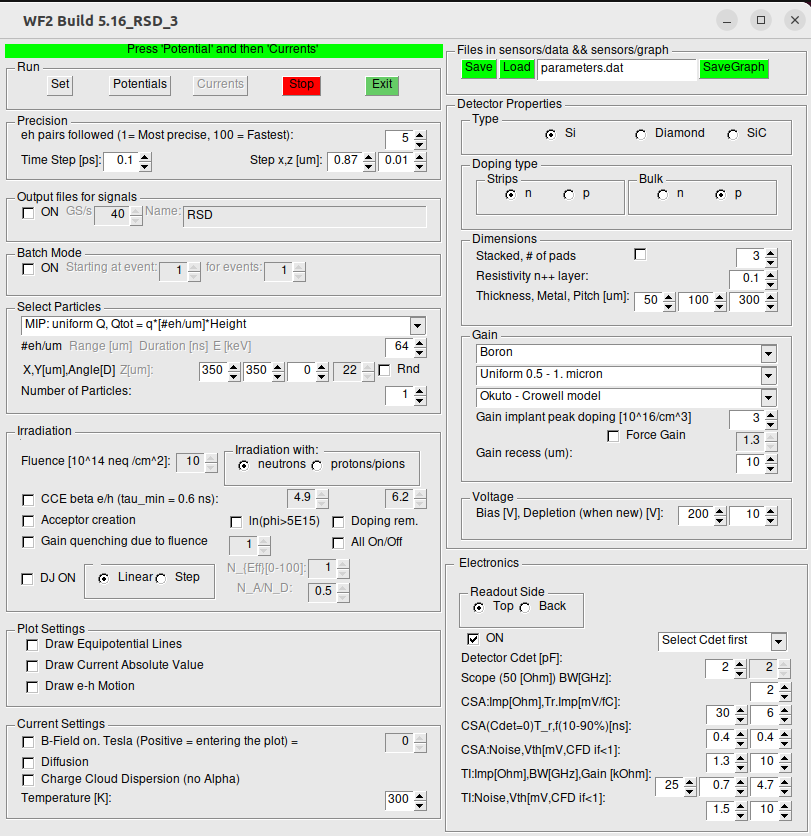
\includegraphics[width=3in]{Images/n_resistivity_other_settings.png}
        \caption{}
        \label{fig:n_resistivity_other_settings}
    \end{subfigure}%
    \begin{subfigure}[t]{0.49\textwidth}
        \centering
        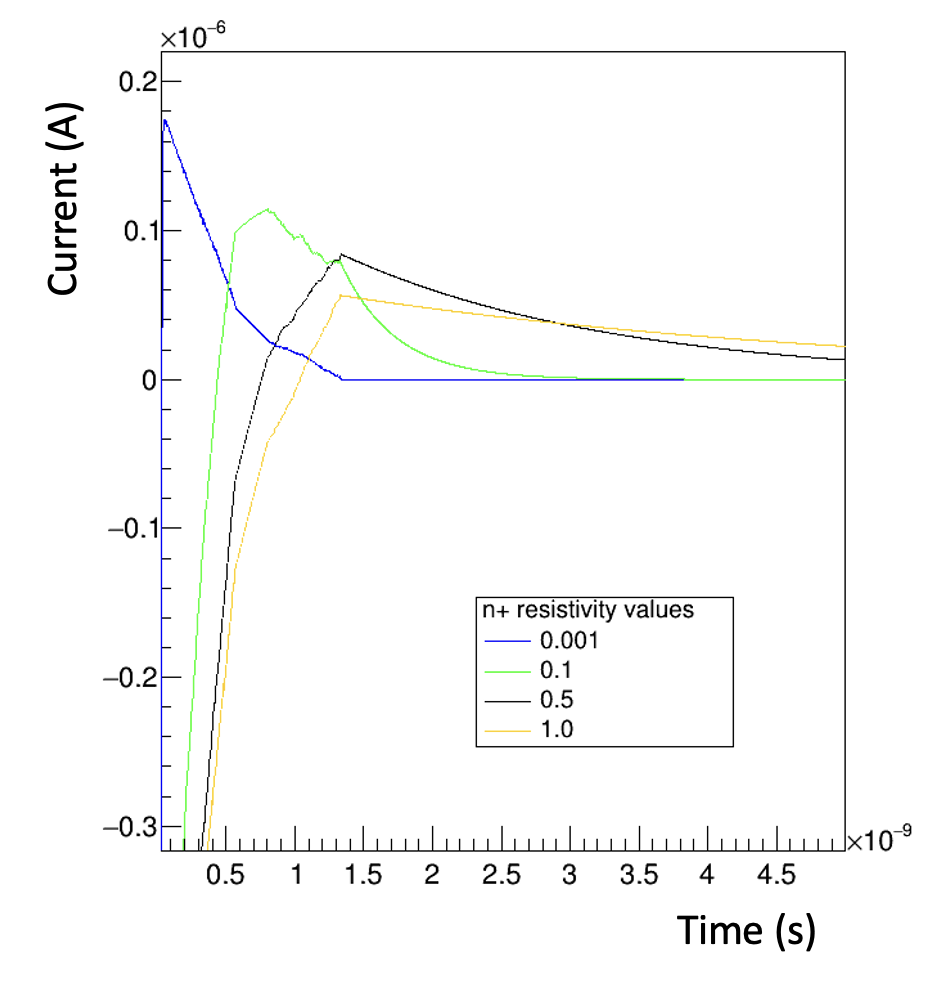
\includegraphics[width=3in]{Images/n_resistivity_plot.png}
        \caption{}
        \label{fig:n_resistivity_plot}
    \end{subfigure}
    \caption{(a) An image of the settings used for the study and (b) the plot of the compiled results obtained as part of this study. As seen, four different values of n+ resistivity was used: 0.001, 0.1, 0.5, and 1.}
    \label{fig:n_resistivity}
\end{figure*}

\hlyellow{Another point to note is that WF2-RSD produced a non-intuitive result for resistivity value = 0.0001. The positive lobe of the signal had a much larger amplitude than those of the other resistivity values.}

\subsection{Thickness}
Amongst the early silicon sensors (that had no gain layer), the thickness did not affect the amplitude of the signal because of two factors contributing to this property: the number of initial charges produced is proportional to the thickness, and the weighting field is inversely proportional to the thickness. In AC-LGADs however, things are not so simple. The simulation results showed that the amplitude/height of the first lobe is inversely proportional to the thickness. That said, the first lobe of the signal broadens for thicker detectors which is expected as the holes generated in the active volume will need longer time to traverse a larger distance.

\begin{figure*}[h!]
    \centering
    \begin{subfigure}[t]{0.49\textwidth}
        \centering
        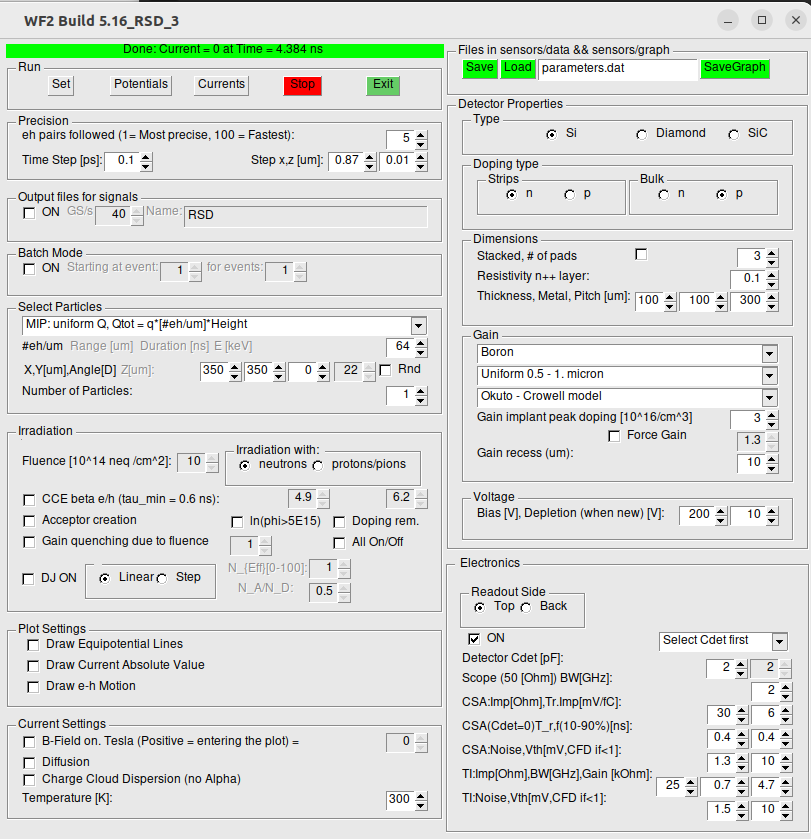
\includegraphics[width=3in]{Images/thickness_other_settings.png}
        \caption{}
        \label{fig:thickness_other_settings}
    \end{subfigure}%
    \begin{subfigure}[t]{0.49\textwidth}
        \centering
        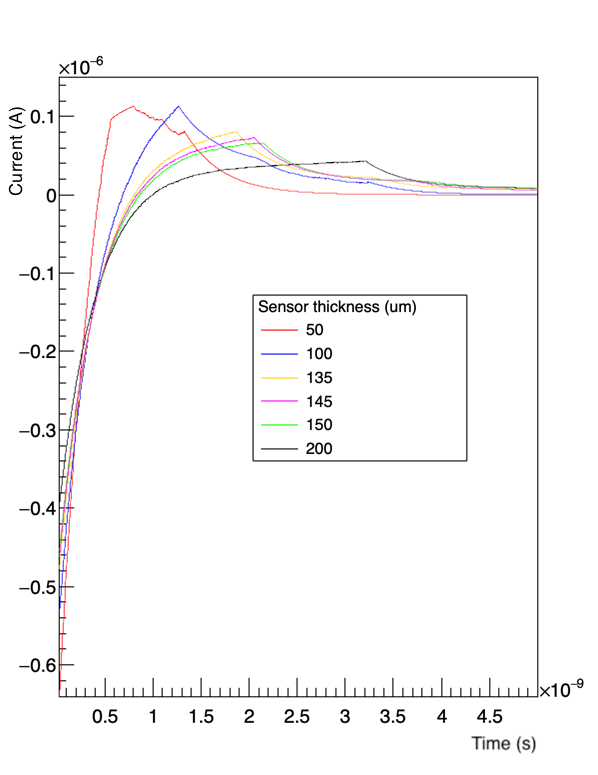
\includegraphics[width=3in]{Images/thickness_plot.png}
        \caption{}
        \label{fig:thickness_plot}
    \end{subfigure}
    \caption{(a) An image of the settings used for the study and (b) the plot of the compiled results obtained as part of this study. As seen, four different values of thicknesses was used: 50, 100, 135, 145, 150, and 200 $\mu$m.}
\end{figure*}

This study was done for thicknesses in steps of 50 $\mu$m, but the reason for looking at 135 $\mu$m and 145 $\mu$m is that alongwith thickness, there was a parallel study on the maximum electric field's variation with thickness. A numerical fluctuation-like effect (probably due to mesh-effects) was observed for the maximum field value around thickness = 150 $\mu$m. The corresponding plot is shown below in Figure \ref{fig:maxEF_vs_thickness}

\begin{figure}
    \centering
    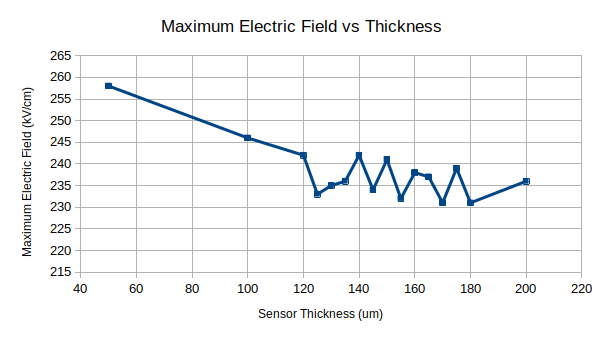
\includegraphics[width=3in]{Images/maxEF_vs_thickness.png}
    \caption{A plot of maximum electric field observed in the sensor for different thicknesses.}
    \label{fig:maxEF_vs_thickness}
\end{figure}

\subsection{Pitch}
The currents seen by the AC-pads for different pitches (and simultaneously maintaining the incident position of the charged particle to be at the center of 4 pads always) was simulated. As expected, the signals seen by four closest pads were the same as the sharing fraction remains the same. The motive of this study (and this was just a shot in the dark owing to the unlikeliness of the desired result) was to reach a limit where the resistance is of a lesser impedance value than that of the capacitive oxide. Reaching this limit would have implied all current goes to the DC contact and would not have any current going through the AC pads, and for the values the simulations were performed over, this limit was not reached. However, the results obtained still are as expected in that the signal sharing fractions would not change for the four nearby pads because the incident particle is in the middle of the four pads. Some images form this study are shown in Figure \ref{fig:varying_pitch}. This study was performed for pitches = 220, 300, 350 and 400 $\mu$m, and 220 $\mu$m instead of 200 $\mu$m was chosen because the pad diameter was set as 200 $\mu$m.

\begin{figure*}[h!]
    \centering
    \begin{subfigure}[t]{0.49\textwidth}
        \centering
        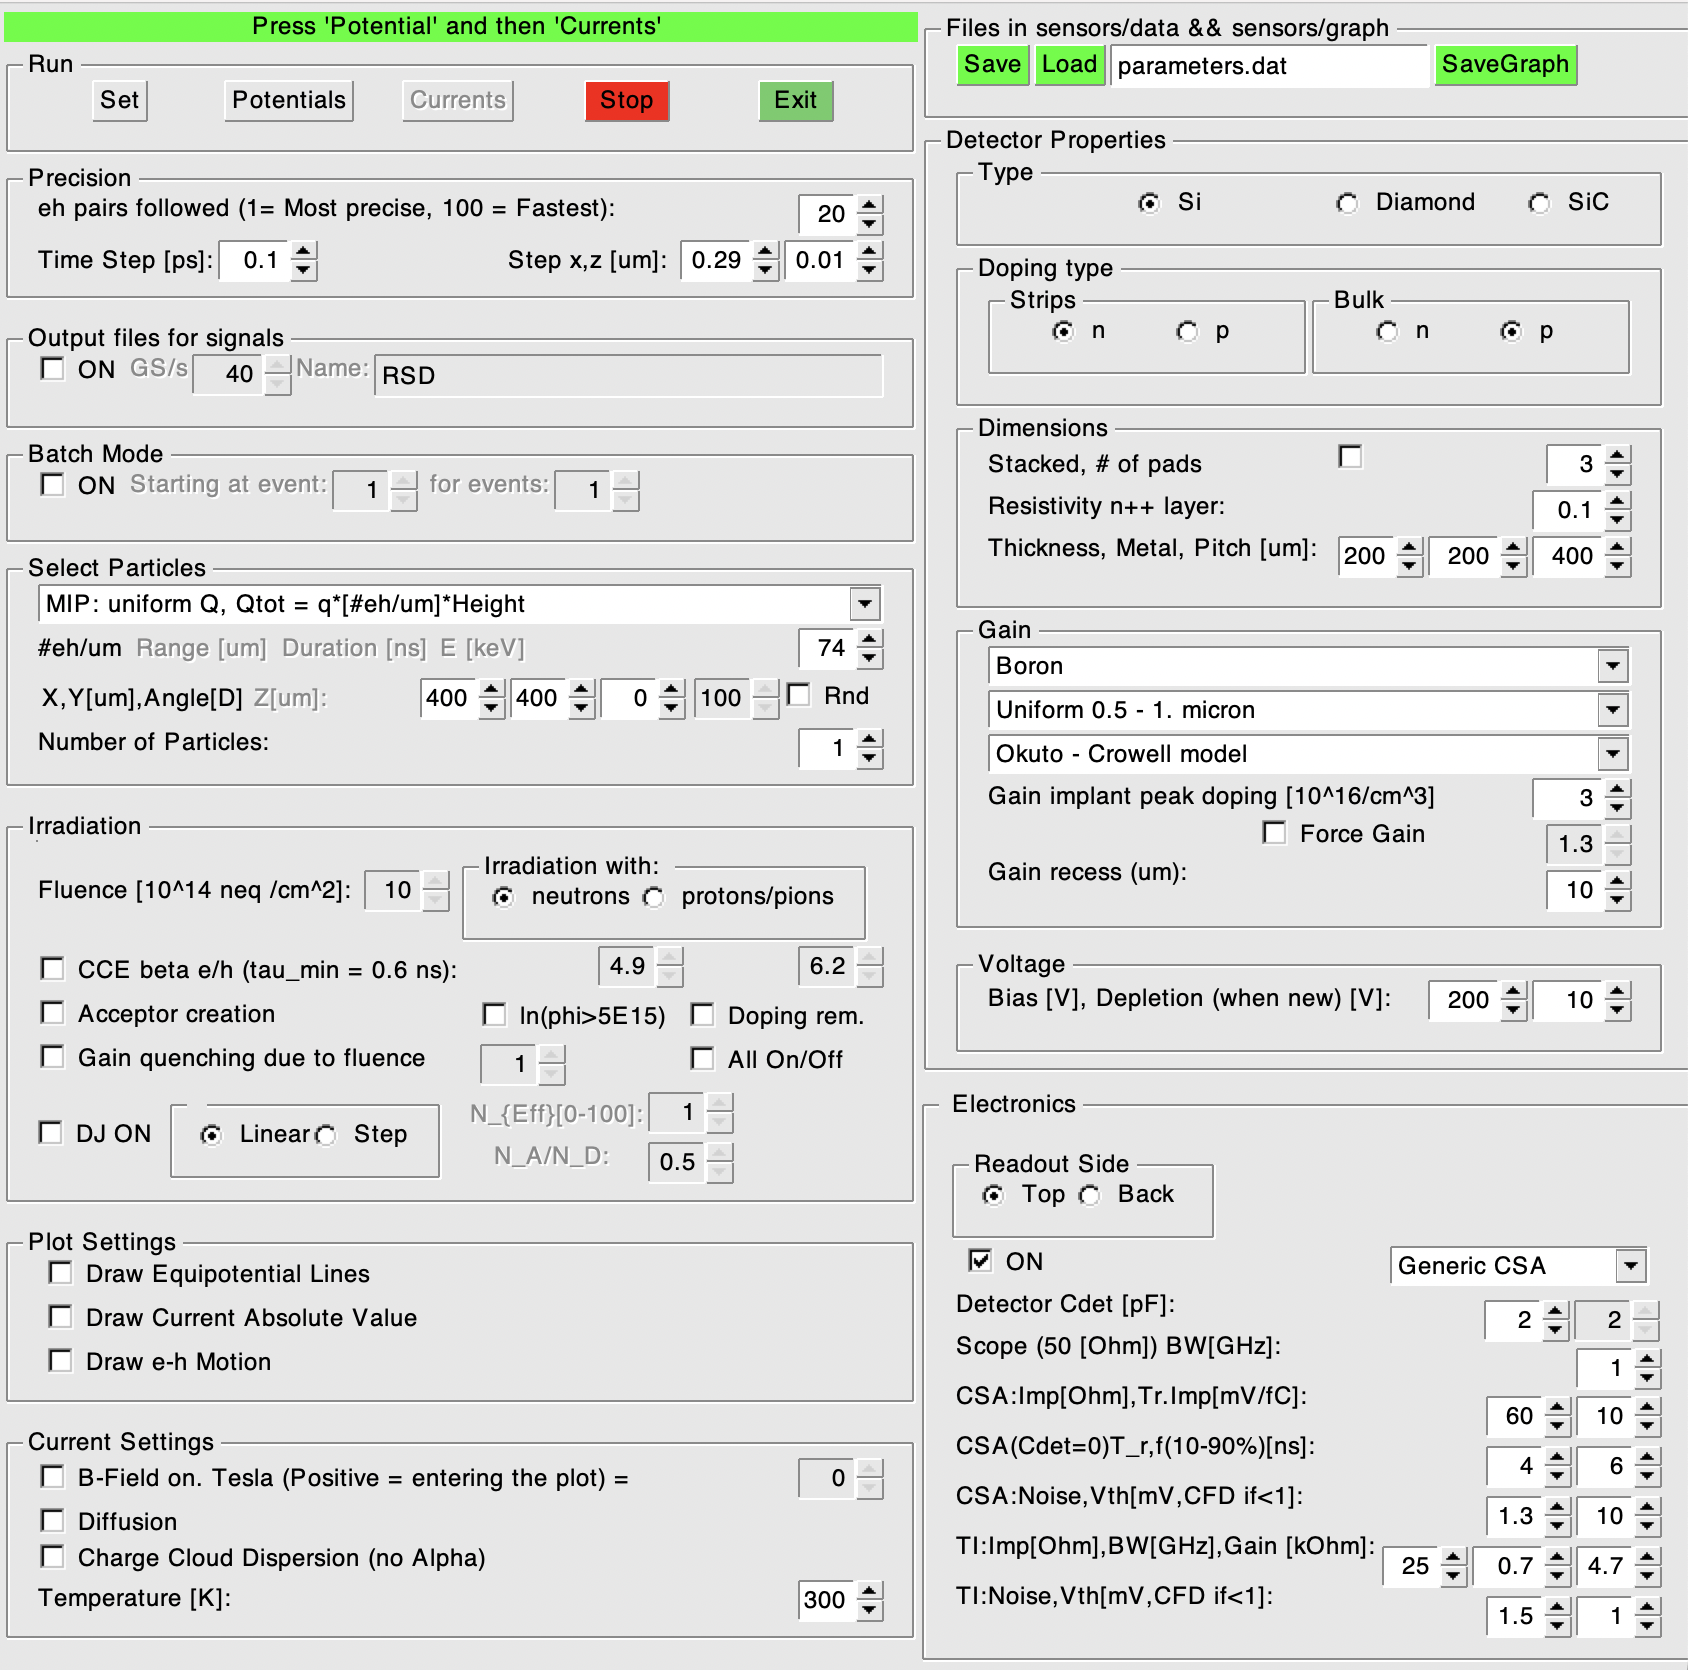
\includegraphics[width=3in]{Images/varying_pitch_other_settings.png}
        \caption{}
        \label{fig:varying_pitch_other_settings}
    \end{subfigure}%
    \begin{subfigure}[t]{0.49\textwidth}
        \centering
        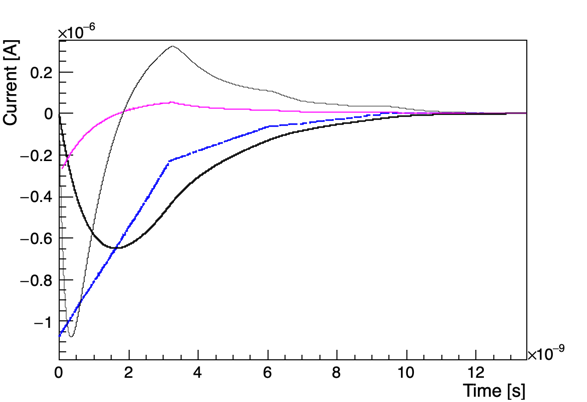
\includegraphics[width=3in]{Images/varying_pitch_300umcase_plot.png}
        \caption{}
        \label{fig:varying_pitch_plot}
    \end{subfigure}
    \caption{(a) An image of the settings used for the study and (b) the electronic response plot for one of the pitch (=300 $\mu$m) values considered.}
    \label{fig:varying_pitch}
\end{figure*}

\subsection{Time delay from hit position}
Depending on where the incident particle hits the sensor, the signal takes a finite non-zero time taken to reach the electronics. This arises due to the time needed by the charges to reach the electrode, or more specifically, the wirebond. In a centimeter-scale AC-LGAD paper \cite{madrid2023}, it was reported that for farther hit positions on the strip from the wirebond, the time delay increases. Simulations were done for pad diameters (200, 300, 400, and 450 $\mu$m) and varying y-coordinates (100, 150, 200, 250, and 600 $\mu$m) for the same x-coordinate (20$\mu$m away from the end of the pad). Although the terminal prints a number for the delay, this is calculated by the LogA model for signal sharing and the objective of this study was to observe the physics simulation to naturally introduce time delays in waveforms for AC pads of different dimensions. This time delay would be arising from the non-zero time taken by the charges travelling through the electrode to reach the wirebond. In WF2-RSD, the current and electronic response of a sensor was simulated for different hit positions (in the gap region). A conclusive correlation between this time-delay and distance from the center of the pads to the incident position, was not found. This statement could atleast be made only for the geometries that was tried. It could be the case that the strips displaying this behavior in the above stated paper were of larger order of lengths, hence this effect might not be prominent in smaller pad sizes. The source code also does not have scope to perform this calculations for this kind of a mechanism.

\begin{figure*}[h!]
    \centering
    \begin{subfigure}[t]{0.49\textwidth}
        \centering
        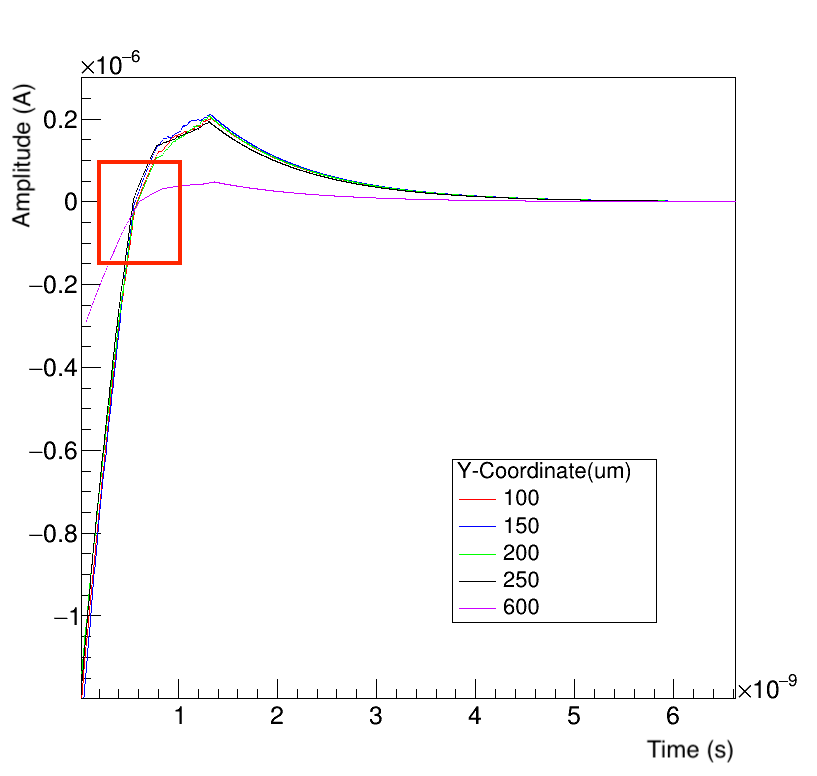
\includegraphics[width=3in]{Images/time_delay_plot_200W_full.png}
        \caption{}
        \label{fig:time_delay_plot_full}
    \end{subfigure}%
    \begin{subfigure}[t]{0.49\textwidth}
        \centering
        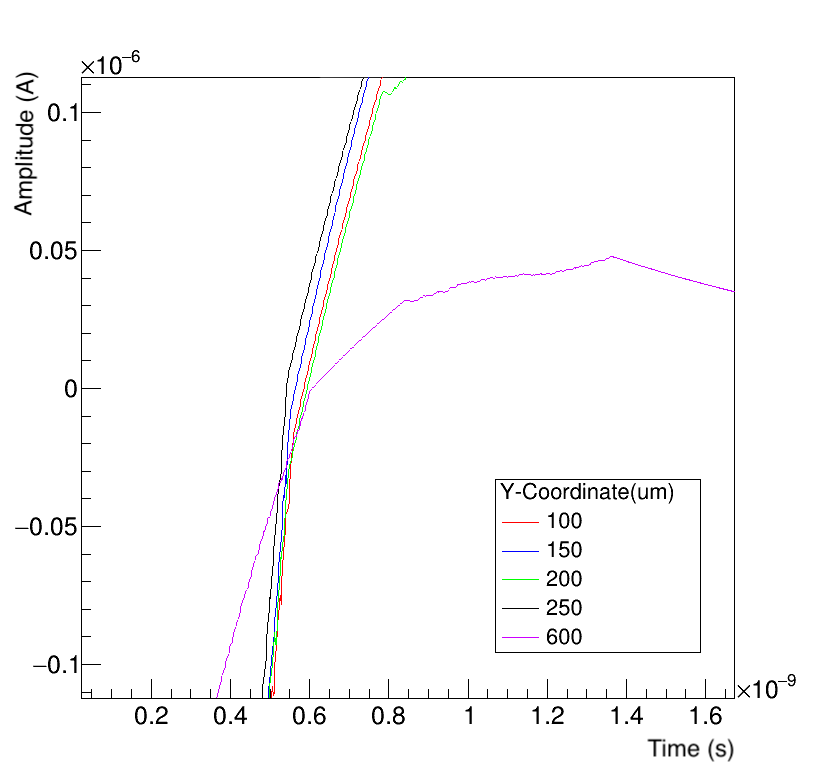
\includegraphics[width=3in]{Images/time_delay_plot_200W_sig.png}
        \caption{}
        \label{fig:time_delay_plot_sig}
    \end{subfigure}
    \caption{A plot of the signals from a sensor with 50 um thickness, 500 um pitch, 200 um pad width for different incident hit positions (same x-coordinate, but different y-coordinates) in the gap region. The red box in Figure (a) corresponds to the region enlarged to produce Figure (b)).}
\end{figure*}

\subsection{Coupling capacitance: pad size}
There are two ways to vary coupling capacitance: varying the diameter of the pads (on the front panel (GUI) of the software) and by varying the oxide layer thickness. Changing geometry is known to introduce other effects like inter-strip capacitance so the former method wouldn't be a proper reductionist study. The details of the second way to vary coupling capacitance (by varying the thickness of the oxide layer) will be discussed in Section \ref{sec:varying-ccp-code}. The results of this study are shown in Figure \ref{fig:varying_pad_size}. We see that smaller pads offer a path of greater impedance so more current reached the DC terminal than the AC pads. Another inference from Figure \ref{fig:varying_pad_size} is that since smaller pads have smaller capacitance, the tails of the second lobe will also have be smaller.

\begin{figure*}[h!]
    \centering
    \begin{subfigure}[t]{0.49\textwidth}
        \centering
        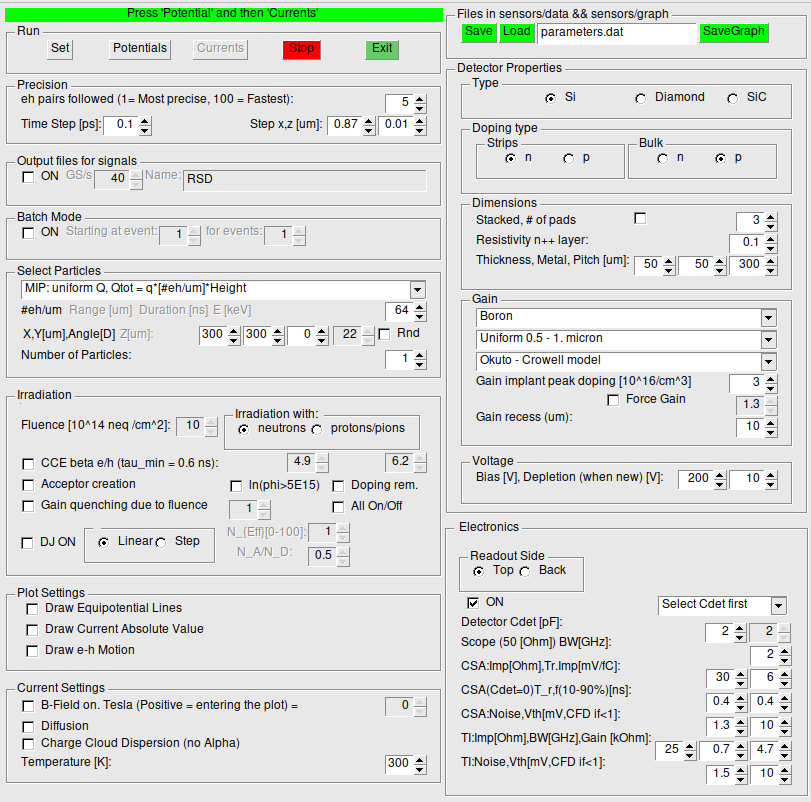
\includegraphics[width=3in]{Images/pad_size_other_settings.png}
        \caption{}
        \label{fig:pad_size_other_settings}
    \end{subfigure}%
    \begin{subfigure}[t]{0.49\textwidth}
        \centering
        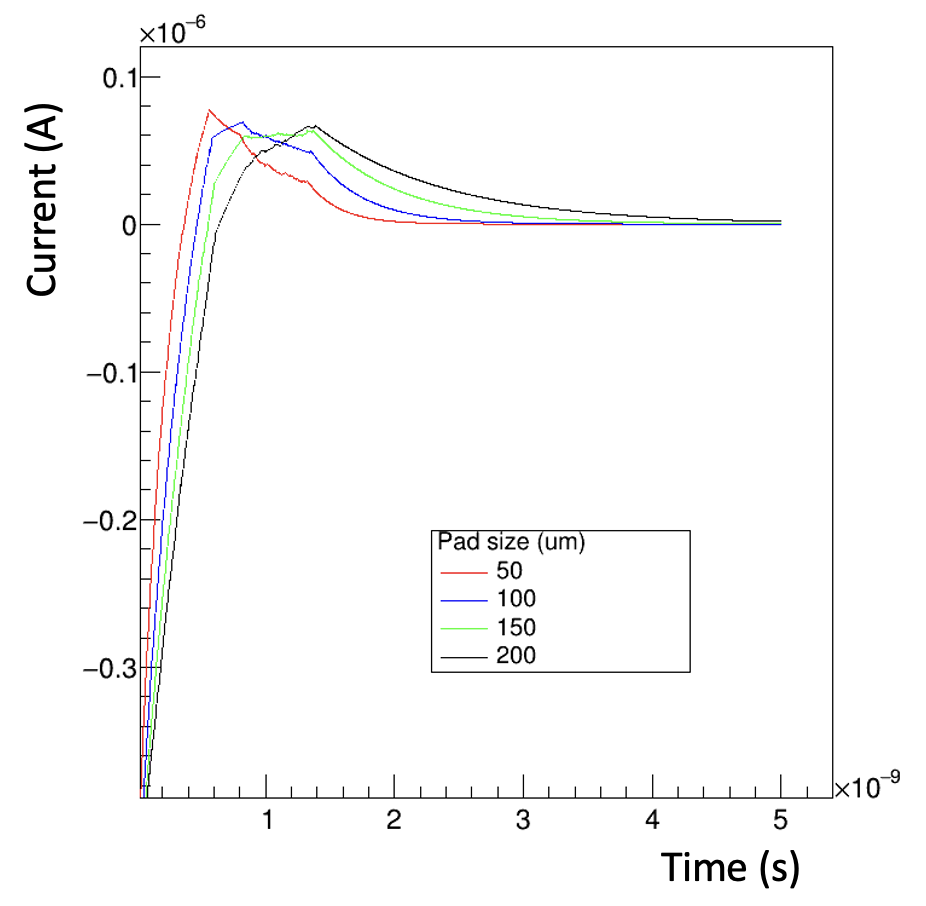
\includegraphics[width=3in]{Images/pad_size_plot.png}
        \caption{}
        \label{fig:pad_size_plot}
    \end{subfigure}
    \caption{(a) An image of the settings used for the study and (b) the plot of the compiled results obtained as part of this study. As seen, four different values of pad diameters was used: 50, 100, 150, and 200 $\mu$m.}
    \label{fig:varying_pad_size}
\end{figure*}

\subsection{Coupling capacitance: capacitance/area of oxide layer - an attempt to reproduce experimental results}\label{sec:varying-ccp-code}
An article \cite{kita2023} reported results on the dependence of signal amplitude for different capacitances for pixel-electrode AC-LGADs.  For this study, a sensor of pitch 150 $\mu$m and square pad of width 140 $\mu$m was used and the subsequent plot the authors obtained is shown in Figure \ref{fig:kita_amp_vs_ccp}.

\begin{figure*}[h!]
    \centering
    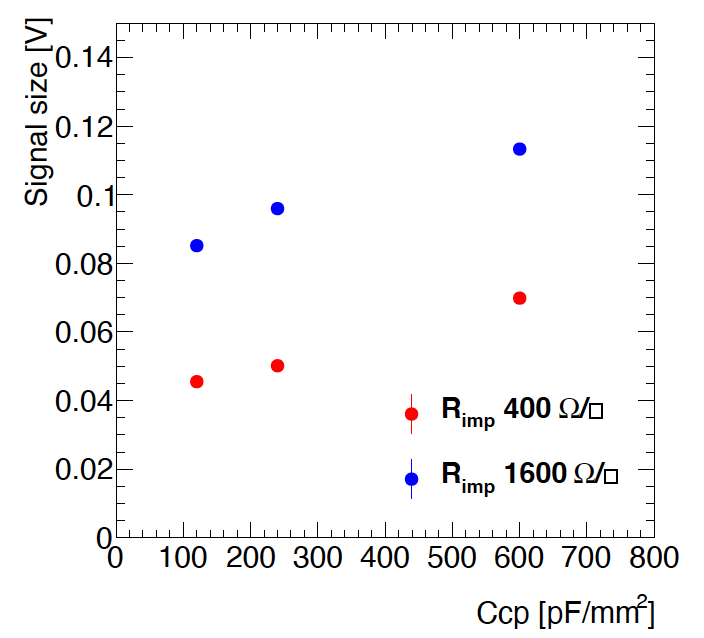
\includegraphics[width=3in]{Images/kita_amp_vs_ccp.png}
    \caption{The signal size evaluated using $^{90}$Sr as a function of C$_{cp}$. Each colored point corresponds to fixed sheet resistance value. Source: \cite{kita2023}}
    \label{fig:kita_amp_vs_ccp}
\end{figure*}

As mentioned earlier, a way to change the coupling capacitance without changing the electrode geometry is by varying the oxide layer thickness, which translates to changing the capacitance/area value of the oxide layer in the source code. Using the similar parameter values used in the article, an attempt was made to recreate the same plot using WF2-RSD. The only unknown was the doping concentration of the gain layer, which was not mentioned in the paper, thus this quanitity was set to close to WF2-RSD's default value. The settings used and the results thus obtained is shown in Figure \ref{fig:recreate_kita_amp_vs_ccp}. It is worth mentioning that for this study, 100 events were simulated in the batch mode, and each event had one MIP traversing through the detector depositing charge according to a Landau distribution.

The documentation for the simulation tool is not present for the RSD version of WF2 but we believe that the variable named \texttt{rsdc1} (that is brought up in calculating the time constants (RC)) found in the Carriers.cxx file is related to the capacitance/area quantity. The signal size (from the AC pads) for different values of \texttt{rsdc1} was simulated and the plot thus obtained is shown in Figure \ref{fig:recreate_kita_amp_vs_ccp}.

\begin{figure*}[h!]
    \centering
    \begin{subfigure}[t]{0.49\textwidth}
        \centering
        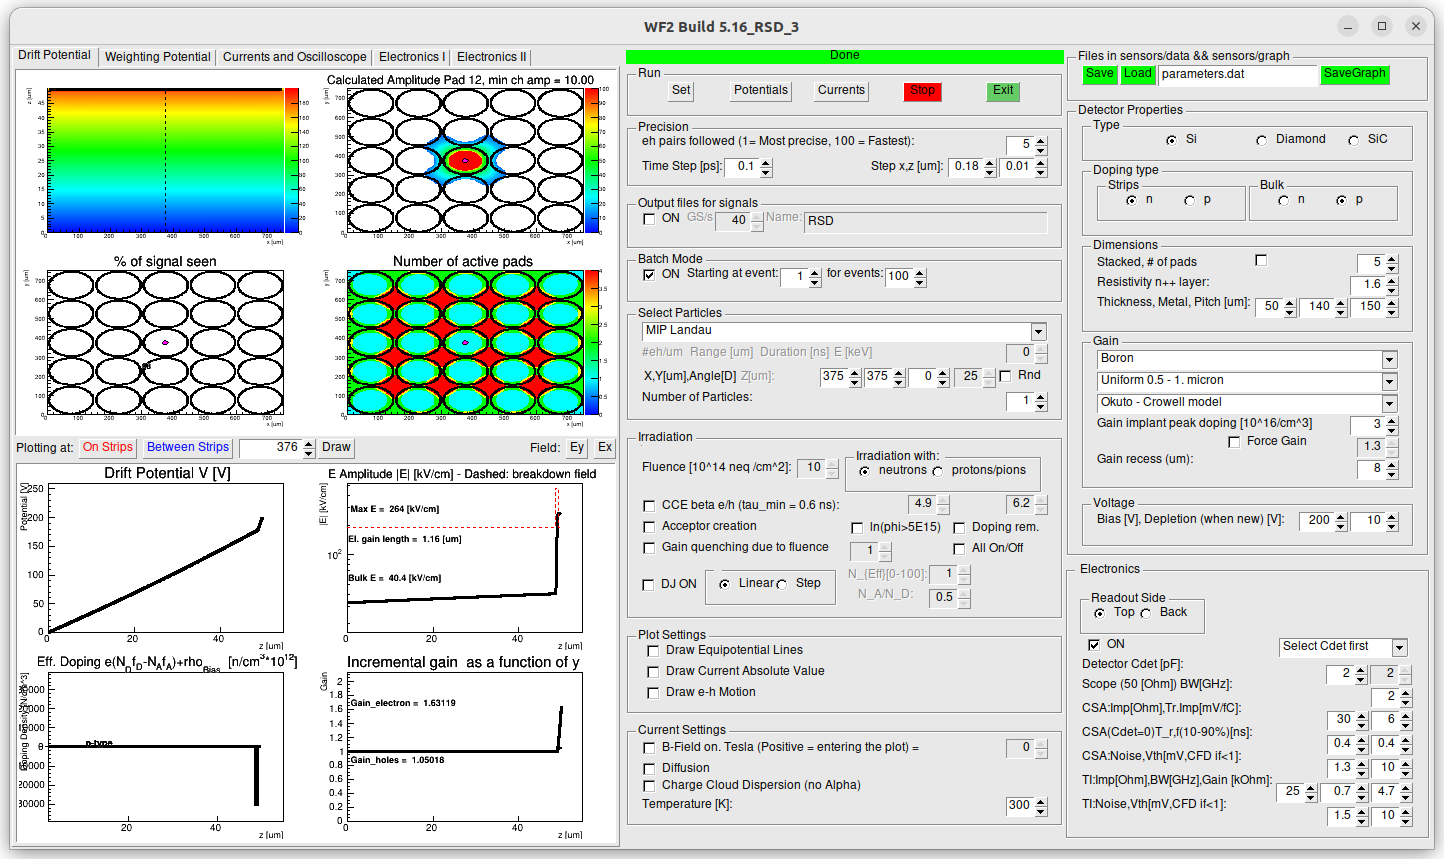
\includegraphics[width=3in]{Images/recreate_kita_amp_vs_ccp_other_settings.png}
        \caption{}
        \label{fig:recreate_kita_amp_vs_ccp_other_settings}
    \end{subfigure}%
    \begin{subfigure}[t]{0.49\textwidth}
        \centering
        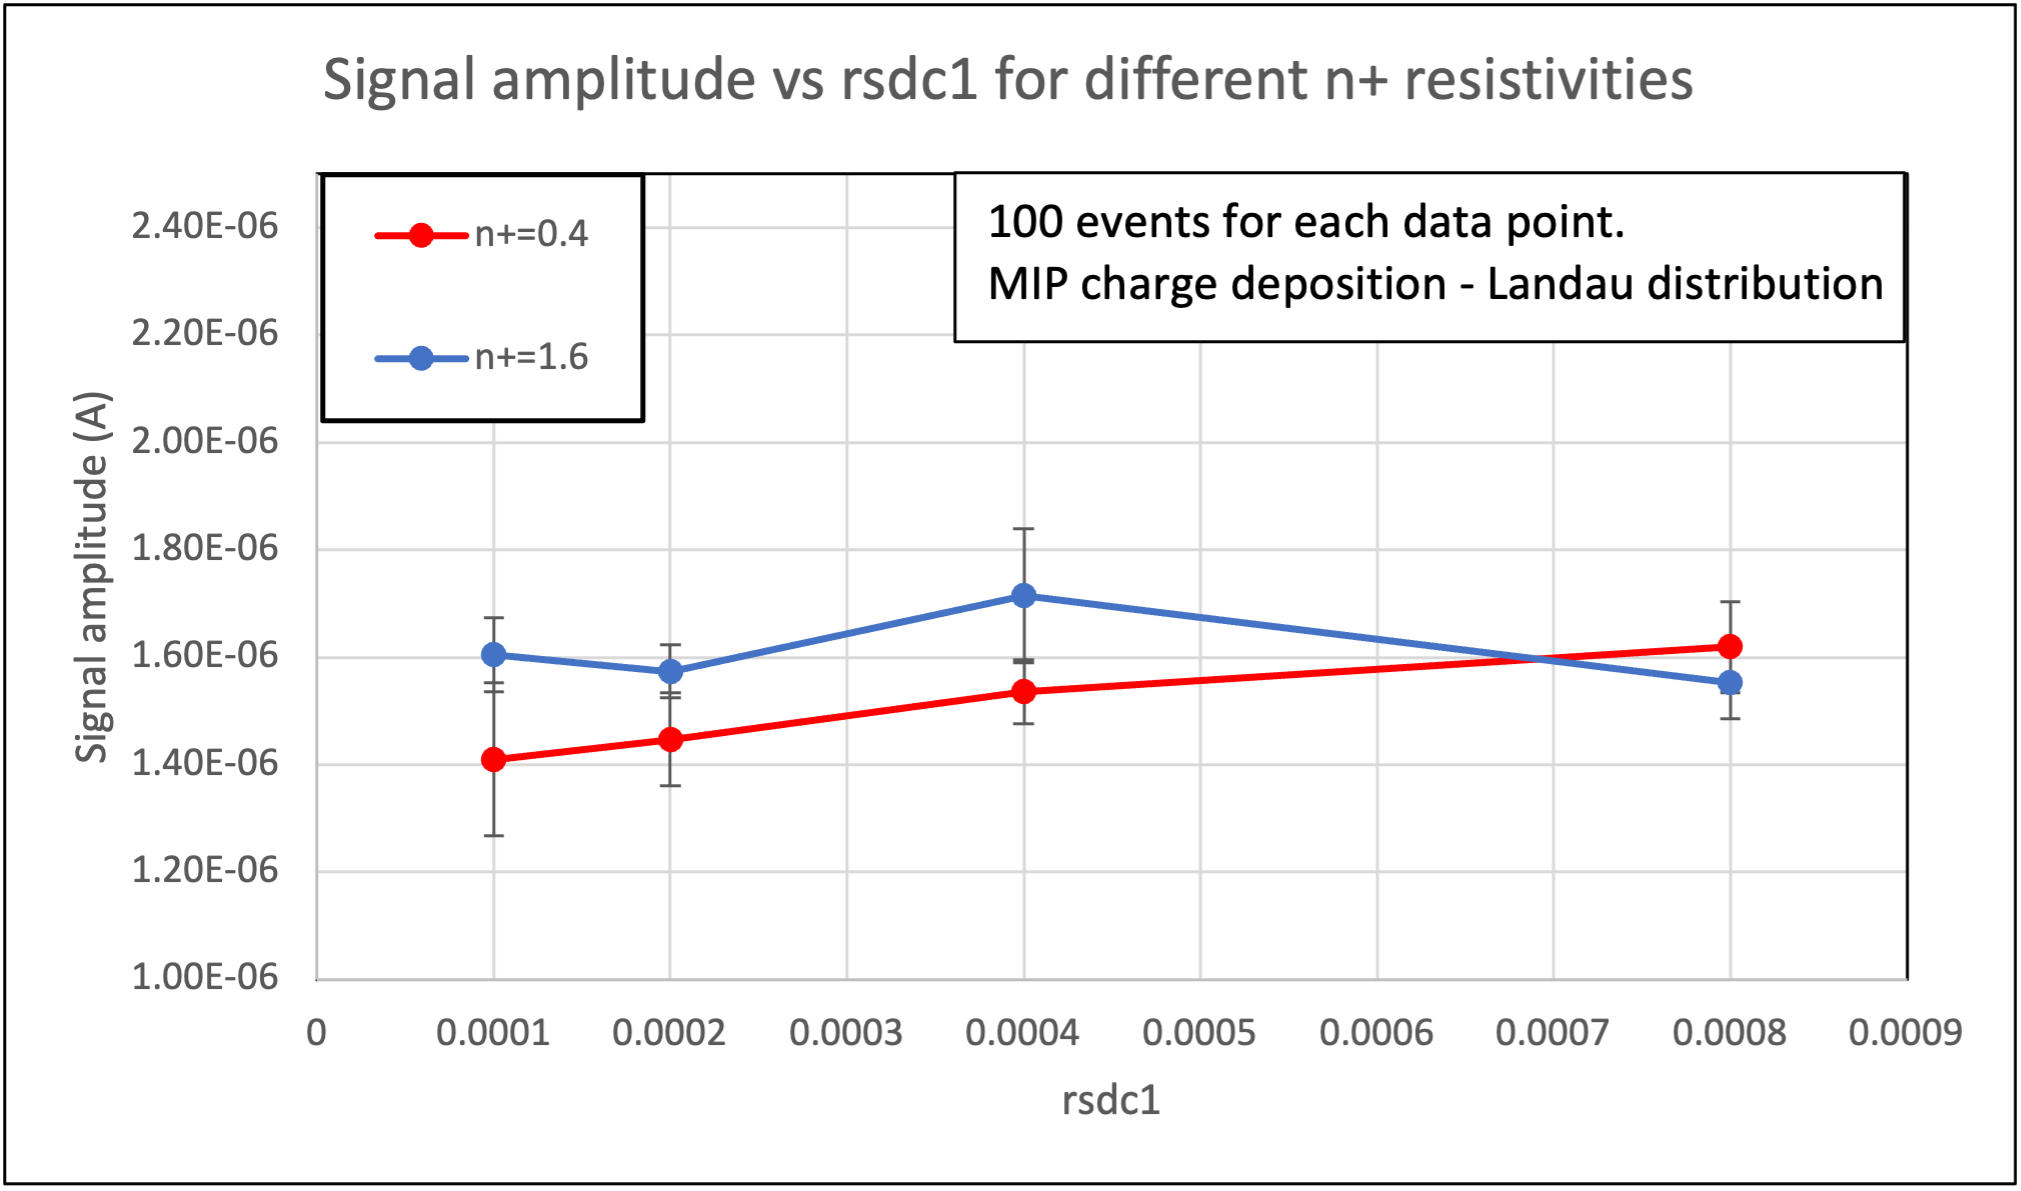
\includegraphics[width=3in]{Images/recreate_kita_amp_vs_ccp_plot.png}
        \caption{}
        \label{fig:recreate_kita_amp_vs_ccp_plot}
    \end{subfigure}
    \caption{(a) An image of the settings used for the study and (b) the plot of the compiled results obtained as part of this study. The X-axis (rsdc1) is the variable in the source code that corresponds to the capacitance/area. \hlyellow{Example: an rsdc1 value of 0.0002 = 200pF/mm$^2$.} The two colored curves correspond to two different sheet resistances (0.4$\equiv$400$\Omega/\square$ and 1.6$\equiv$1600$\Omega/\square$).}
    \label{fig:recreate_kita_amp_vs_ccp}
\end{figure*}

% \subsection{Updates in different versions}
% WF2\_5.4 has another update with regard to choosing AC/DC coupling on the top-readout surface, a feature that WF2\_5.17 does not have. Additionally, some other physics models for the gain layer (which is called as ``gain parameterisation'' in Cartiglia's website) seem to have been added.
% \newline
% That said, WF2-RSD does not have the option to introduced AC-coupling in the readout, so can we not fully simulate AC-LGADs? According to one of Cartiglia's \href{https://indico.cern.ch/event/928957/contributions/3913535/attachments/2069369/3473666/FCCee_Cartiglia.pdf}{slides}, it seems like WF2-RSD is for AC coupled simulations by default.
% \newline
% I still have not deeply looked at the differences in WF2-RSD between version 5.15 and version 5.16.

\bibliography{references}

\end{document}